\begin{frame}
	\frametitle{About Kilobots}
	\begin{columns}
		\begin{column}{0.4\textwidth}
			\begin{figure}
				\centering
				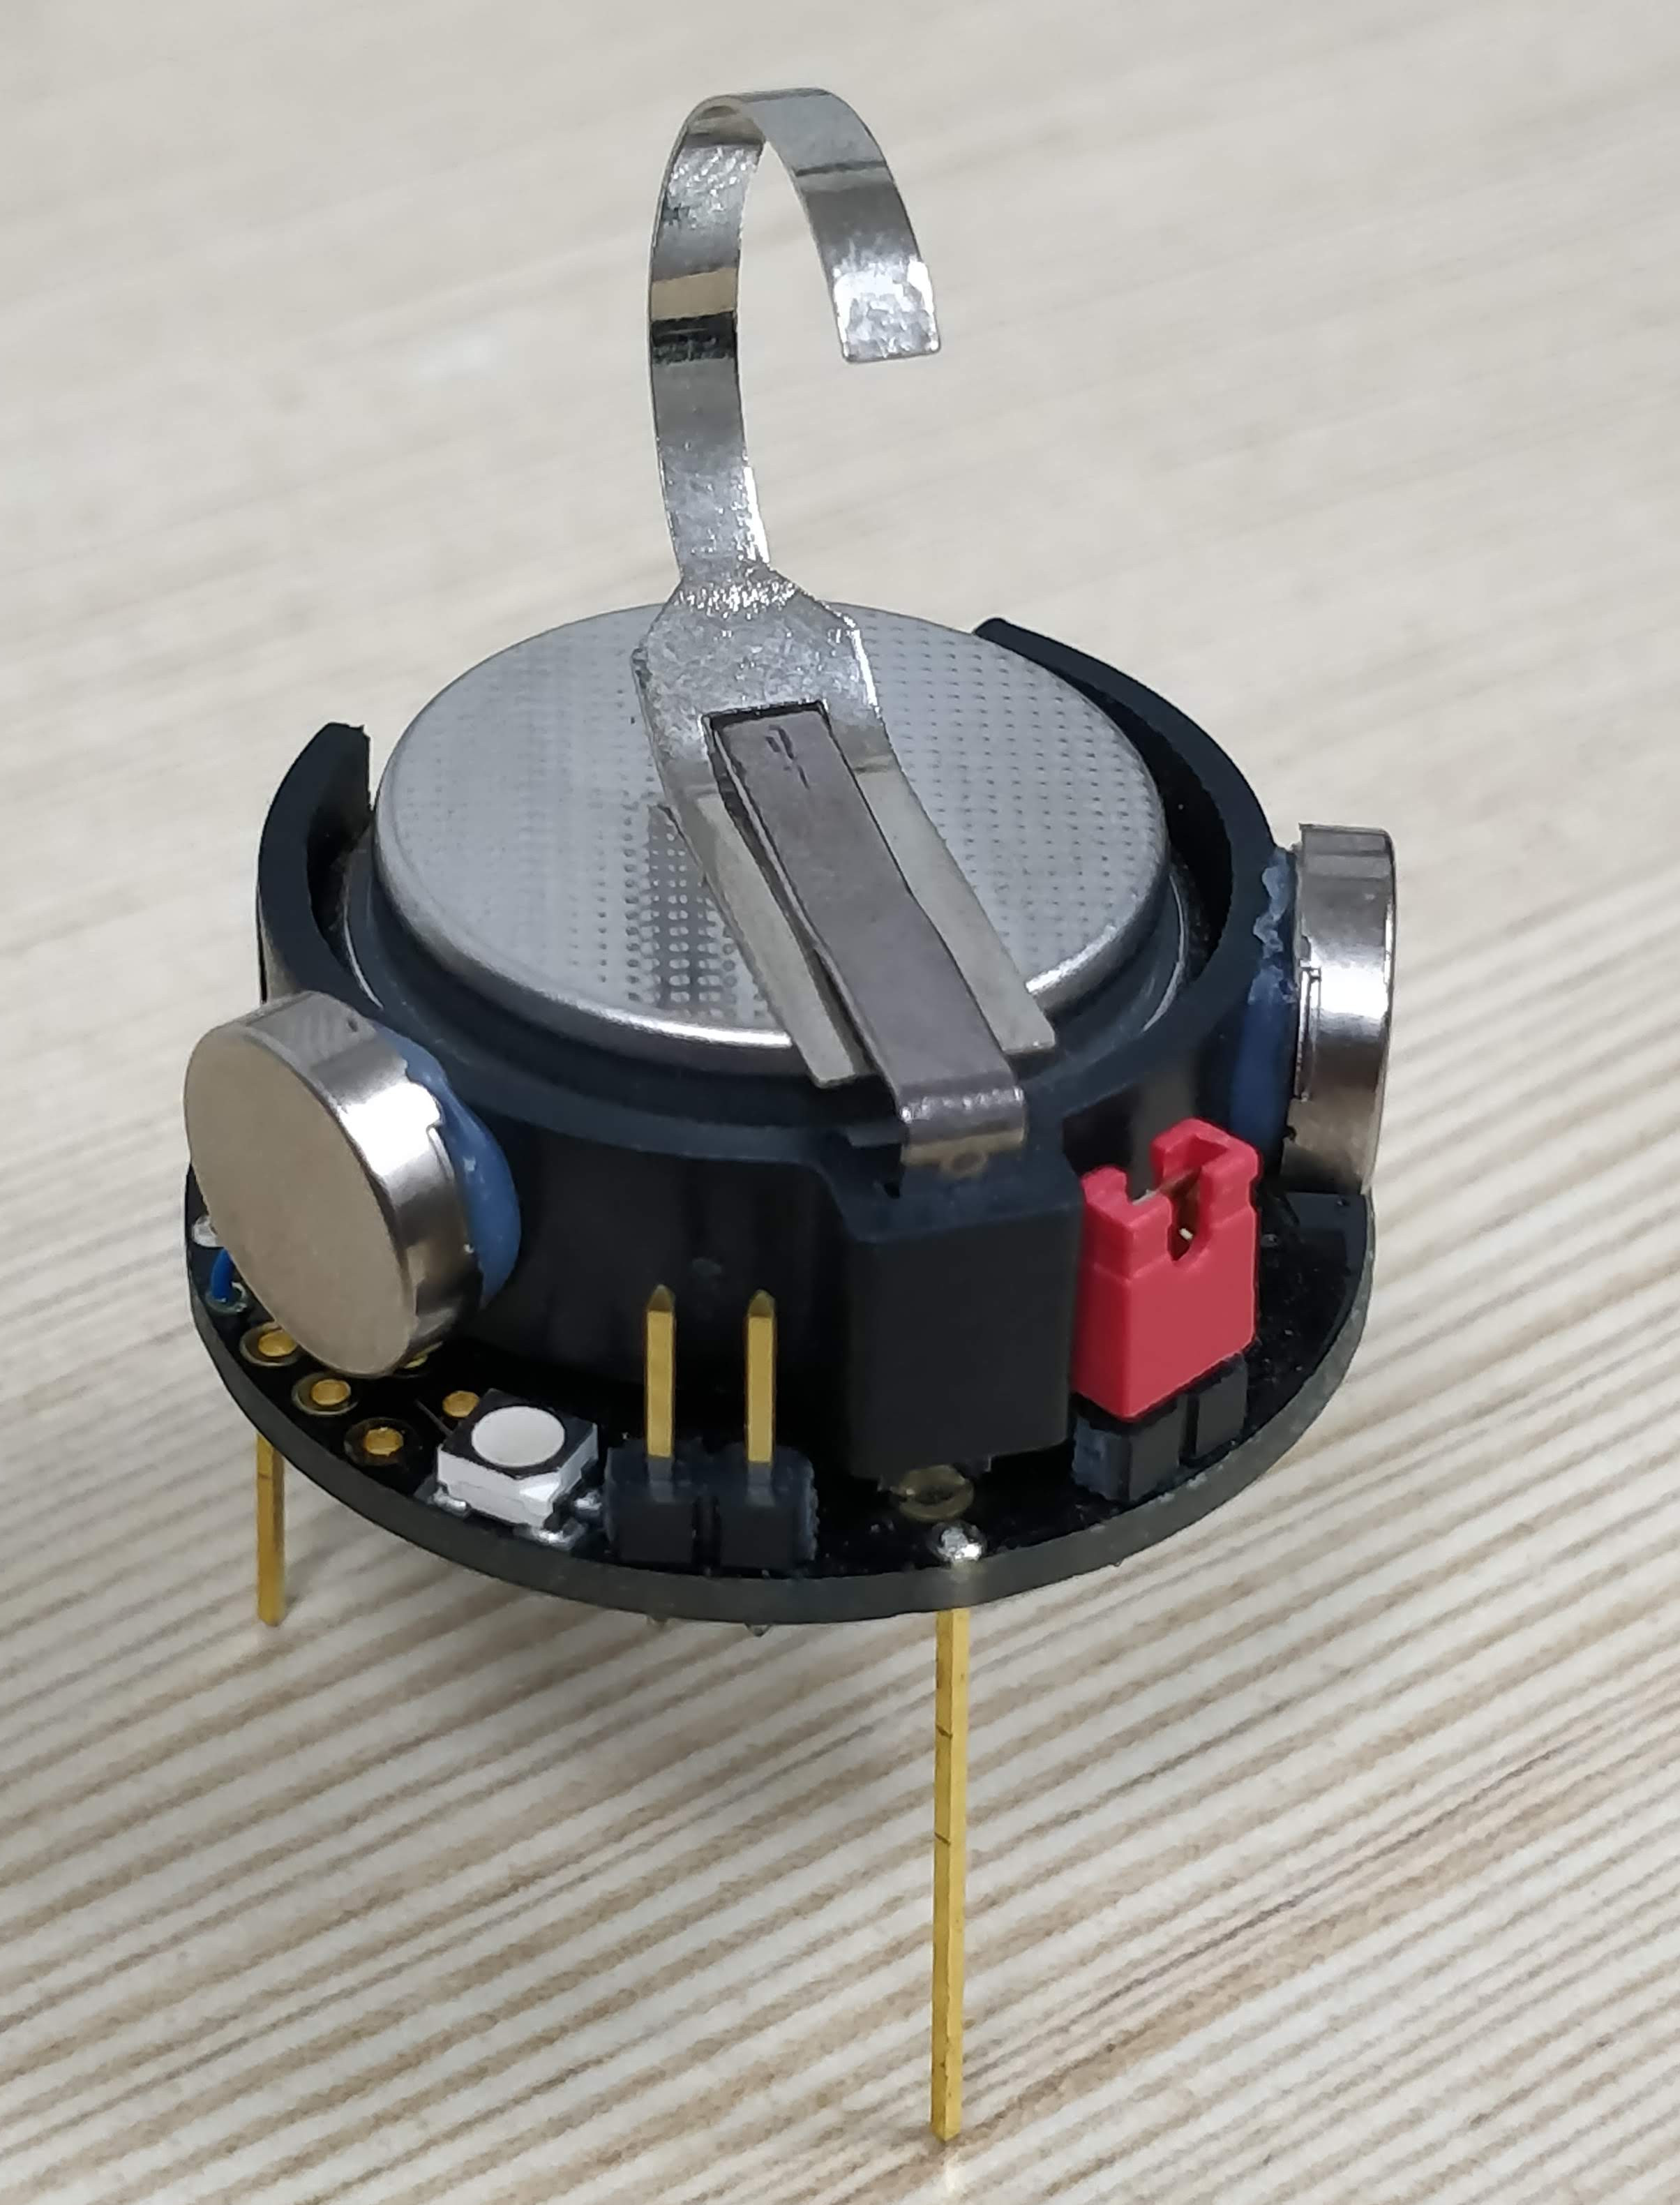
\includegraphics[scale=0.05]{kilobots}
				\caption{Kilobot}
			\end{figure}
		\end{column}
						
		\begin{column}{0.45\textwidth}
			\begin{itemize}
				\item ATmega 328p processor 
				\item Li-Ion 3.7V battery 
				\item IR sensor 
				\item Light sensor 
				\item Vibration motors (1 cm/sec, 45 degrees/sec)
			\end{itemize}
		\end{column}
	\end{columns}
\end{frame}

\begin{frame}
	\frametitle{About Kilobots}
	\begin{columns}
		\begin{column}{0.4\textwidth}
			\begin{figure}
				\centering
				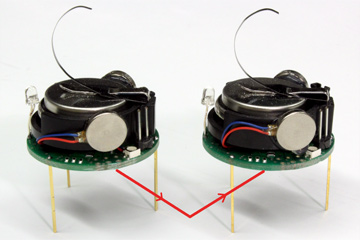
\includegraphics[scale=0.4]{comm}
				\caption{Communication between two Kilobots}
			\end{figure}
		\end{column}
						
		\begin{column}{0.45\textwidth}
			\begin{itemize}
				\item Reflecting IR light
				\item Communication up to 7 cm (32kb/s) away 
				\item Using over-head controller
			\end{itemize}
		\end{column}
	\end{columns}
\end{frame}

\begin{frame}
	\frametitle{Channel use by Kilobots}
	\begin{itemize}
		\item All robots using IR Channel
		\item CSMA-CA method 
		\item Reduction of Channel bandwidth        
	\end{itemize}
\end{frame}
